% A graph representing a city with the weight of the roads between each pair of nodes (location).

\documentclass[]{standalone}

\usepackage{tikz}
\usepackage{fontawesome5}
\usepackage{xcolor}

\begin{document}

\begin{tikzpicture}

	\node[draw, circle, thick] (orange) at (0, 0) {\color{orange}\faHome};

	\node[draw, circle] (green) at (2, 0) {\color{green}\faHome};

	\node[draw, circle] (blue) at (1.5, 1.3) {\color{blue}\faHome};

	\node[draw, circle, thick] (red) at (3, 1) {\color{red}\faHome};

	\node[draw, circle] (purple) at (3, -1) {\color{purple}\faHome};

	% Edges with weights (km)

	\draw[-, red, thick] (orange) to [bend right] node[above, black] {2} (green);
	\draw[-, red, thick] (green) to [bend right] node[right, black] {1} (blue);
	\draw[-, red, thick] (blue) to [bend left] node[above, black] {3} (red);
	\draw[-] (red) to [bend left] node[right] {4} (purple);
	\draw[-] (orange) to [bend left] node[above] {4} (blue);
	\draw[-] (green) to [bend right] node[left] {1.5} (purple);

\end{tikzpicture}

\end{document}